\chapter[Predictive control of a CSR]{Constrained, explicit predictive control for current source buck-type rectifiers}\label{EMPC:sec:main}

As mentioned in section \ref{BASICCSR:sec:CSR} current source rectifiers (CSR) play a major role in industrial instrumentation. They are invaluable, in the fields of direct power control, torque control, or power injection is required. In this chapter, the modeling and control of such CSR (or buck-type rectifiers), in a model based predictive manner, with explicit partitioning of the state space. The reason of the regular MPC's insufficiency is that power electronic systems require very low time constant to operate smoothly. As such pre-mapping the state-space with applicable control rules gives a great leverage, thus making the possible computational unit much cheaper.
		
\section{Modeling}\label{EMPC:sec:Modeling}

Understandably, model based controllers require the system's model the ought to control, or supervise. In this case the most common structure of a CSR is chosen, with inductive and capacitive filtering on both ends. The differential equations are constructed based on Kirchoff's law and then presented as a state space model for further examination.

\subsection{Mathematical modeling of the CSR}\label{EMPC:sec:ModelofCSR}

    The structure of the classical three phase buck-type current source rectifier (CSR) is presented in \ref{EMPC:fig:network}. In continuous current mode, the differential equations corresponding to the CRS’s inductor currents and capacitor voltages are the following:

    \begin{figure}[!ht]
        \centering
        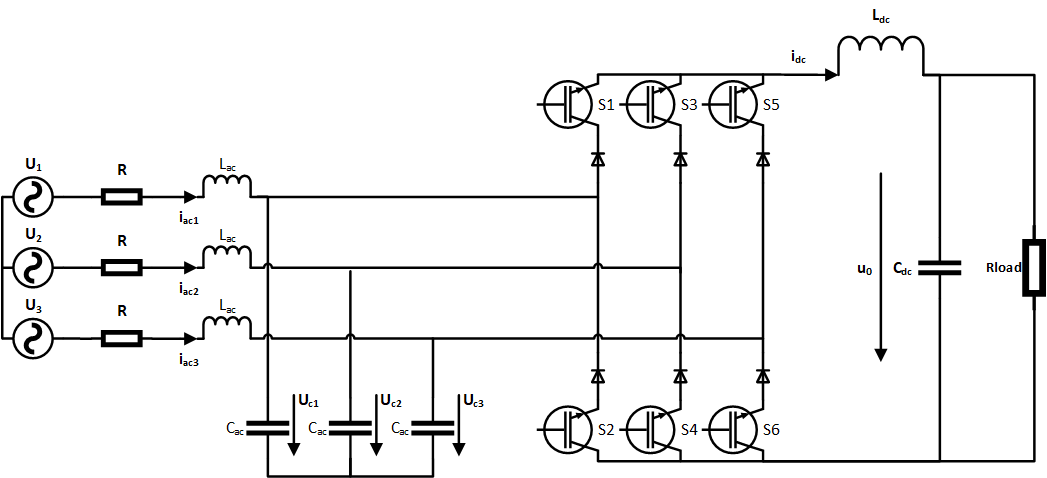
\includegraphics[width=\textwidth]{EMPC_PNG_Pics/circuit.png}
        \caption{Circuit diagram of the three-phase buck-type rectifier with insulated gate bipolar transistors (IGBTs).}
        \label{EMPC:fig:network}
    \end{figure}
		
        \begin{equation}
        \begin{array}{rcl}
            L_{ac}\dot{i_{ac_p}}&=&u_p-u_{c_p}-Ri_{ac_p}\\
            C_{ac}\dot{u_{c_p}}&=&i_{ac_p}-\delta_pi_{dc}\\
            L_{dc}\dot{i_{dc}}&=&(\sum_{p=1}^{3}\delta_pu_{c_p})-u_0\\
            C_{dc}\dot{u_0}&=&i_{dc}-\frac{u_0}{R_{load}}\\
        \end{array}
        \label{EMPC:equ:abc_eqn}
    \end{equation}

    where $p\in\{1,2,3\}$ is the index of three phases and $\delta_p$ describes the conduction state of the rectifier leg p \ref{EMPC:equ:delta_set}.

    \begin{equation}
        \begin{array}{rcl}
            \delta_p&=&\begin{Bmatrix}
                \textrm{1 if the upper transitor is ON}\\
                \textrm{-1 if the lower transistor is ON}\\
                \textrm{0 if both are ON or OFF}
            \end{Bmatrix}
        \end{array}
        \label{EMPC:equ:delta_set}
    \end{equation}

    Converting the components in the stationary (Clarke) frame of the space phasors of the three-phase quantities, from \ref{EMPC:equ:abc_eqn} it results:

    \begin{equation}
        \begin{array}{rcl}
            L_{ac}\dot{i_{ac_\alpha}}&=&u_\alpha-u_{c_\alpha}-Ri_{ac_\alpha}\\
            L_{ac}\dot{i_{ac_\beta}}&=&u_\beta-u_{c_\beta}-Ri_{ac_\beta}\\
            C_{ac}\dot{u_{c_\alpha}}&=&i_{ac_\alpha}-\delta_\alpha i_{dc}\\
            C_{ac}\dot{u_{c_\beta}}&=&i_{ac_\beta}-\delta_\beta i_{dc}\\
            L_{dc}\dot{i_{dc}}&=&1.5(\delta_\alpha u_{c_\alpha}+\delta_\beta u_{c_\beta})-u_0\\
            C_{dc}\dot{u_0}&=&i_{dc}-\frac{u_0}{R_{load}}\\
        \end{array}
        \label{EMPC:equ:abc_alfabeta}
    \end{equation}

    Equation \ref{EMPC:equ:abc_alfabeta} is transformed to the synchronous reference (Park) frame rotating with the $u_{c_d}$ capacitor voltage space vector. The resulting mathematical model is thus:

    \begin{equation}
        \begin{array}{rcl}
            L_{ac}\dot{i_{ac_d}}&=&u_d-u_{c_d}-Ri_{ac_d}+\omega_s L_{ac}i_{ac_q}\\
            L_{ac}\dot{i_{ac_q}}&=&u_d-u_{c_q}-Ri_{ac_q}-\omega_s L_{ac}i_{ac_d}\\
            C_{ac}\dot{u_{c_d}}&=&i_{ac_d}-\delta_di_{dc}+\omega_s C_{ac}u_{c_q}\\
            C_{ac}\dot{u_{c_q}}&=&i_{ac_q}-\delta_qi_{dc}-\omega_s C_{ac}u_{c_d}\\
            L_{dc}\dot{i_{dc}}&=&1.5(\delta_d u_{c_d}+\delta_q u_{c_q})-u_0\\
            C_{dc}\dot{u_0}&=&i_{dc}-\frac{u_0}{R_{load}}\\
        \end{array}
        \label{EMPC:equ:abc_dq}
    \end{equation}

    where $\omega_s$ represents the network voltage vector’s angular velocity.

    \subsection{Model simplification}\label{EMPC:sec:Simplification}

    Notice, that the sixth-order ODE model \ref{EMPC:equ:abc_dq} is bilinear in its states and
    inputs because of the product terms (e.g.: $\delta_di_{dc}$). As such, using design methods for linear systems is not straightforward. The high complexity given by the system’s order is another problem to tackle. For designing classic MPC, linear, low-order equation systems are favorable. Hence simplification of the model would bring noteworthy benefits, making the MPC design more straightforward, when a linear system resulted.
    Since the three phase alternating current (AC) and the direct current (DC) side’s time constants differ significantly (as in the AC: $\omega_{ac}=\frac{1}{\sqrt{L_{ac} C_{ac}}}\cong5.7\cdot10^3$ rad/s, and on the DC: $\omega_{dc}=\frac{1}{\sqrt{L_dc C_dc}}\cong2.8\cdot10^2$ rad/s, see Table \ref{EMPC:tbl:params}. for reference). Thus, the differential equations can be separated into two sets, and the control of the AC and DC sides can be decoupled as described in \cite{ahmed2014model}. The AC side model results as follows:


    \begin{equation}
        \begin{array}{rcl}
            \begin{bmatrix}
                \dot{i_{ac_d}}\\
                \dot{i_{ac_q}}\\
                \dot{u_{c_d}}\\
                \dot{u_{c_q}}
            \end{bmatrix}&=&
            \begin{bmatrix}
                -\frac{R}{L_{ac}}   &\omega &-\frac{1}{L_{ac}}  &0\\
                -\omega   &-\frac{R}{L_{ac}} &0  &-\frac{1}{L_{ac}}\\
                \frac{1}{C_{ac}}   &0 &0  &\omega\\
                0   &\frac{1}{C_{ac}} &-\omega  &0
            \end{bmatrix}
            \begin{bmatrix}
                i_{ac_d}\\
                i_{ac_q}\\
                u_{c_d}\\
                u_{c_q}
            \end{bmatrix}+
            \begin{bmatrix}
                \frac{u_d}{L_{ac}}\\
                \frac{u_q}{L_{ac}}\\
                -\frac{\delta_di_{dc}}{C_{ac}}\\
                -\frac{\delta_qi_{dc}}{C_{ac}}
            \end{bmatrix}
        \end{array}
        \label{EMPC:equ:mtx_AC}
    \end{equation}

    Looking at the state matrix it can be further stated that there are only weak couplings between the $d$ and $q$ synchronous reference frame components. This allows to handle them separately, and later to design separate control for each.
    The equation system describing the DC side dynamics is the following:

    \begin{equation}
        \begin{array}{rcl}
            \begin{bmatrix}
                \dot{i_{dc}}\\
                \dot{u_{0}}
            \end{bmatrix}&=&
            \begin{bmatrix}
                0&  -\frac{1}{L_{dc}}\\
                \frac{1}{C_{dc}}&   -\frac{1}{R_{load}C_{dc}}
            \end{bmatrix}
            \begin{bmatrix}
                i_{dc}\\
                u_0
            \end{bmatrix}+
            \begin{bmatrix}
                \frac{1.5}{L_{dc}}(\delta_du_{c_d}+\delta_qu_{c_q})\\
                0
            \end{bmatrix}
        \end{array}
        \label{EMPC:equ:mtx_DC}
    \end{equation}

    It can be noticed that, with the AC and DC model separation, bilinearity disappears, since the binding coefficients are present only in the input $(\textbf{u})$ of the DC state space model \ref{EMPC:equ:mtx_DC}. Consequently, all equations are linear and with a considerably lower order, making control design much easier and allowing for the application of linear design methods. For the DC side dynamics, the linear time invariant differential equation system’s matrices can be identified for predictive control design purposes:

    \begin{equation}
        \begin{array}{rcl}
            \textbf{x}&=&\begin{bmatrix}
                i_{dc}\\
                u_0
            \end{bmatrix},\\
            \textbf{u}&=&(\delta_d u_{c_d}+\delta_q u_{c_d}),\\
            \textbf{y}&=&u_0,\\
            \textbf{A}&=&\begin{bmatrix}
                0&  -\frac{1}{L_{dc}}\\
                \frac{1}{C_{dc}}&   -\frac{1}{R_{load}C_{dc}}
            \end{bmatrix},\\
            \textbf{B}&=&\begin{bmatrix}
                i_{dc}\\
                u_0
            \end{bmatrix},\\
            \textbf{C}&=&\begin{bmatrix}0 &1\end{bmatrix}.
        \end{array}
        \label{EMPC:equ:mtx_ctrl}
    \end{equation}

    where \textbf{x}, \textbf{u} and \textbf{y} are the state, input and output vectors of the DC-side system, and \textbf{A}, \textbf{B} and \textbf{C} are the state, input and output matrices.
    The circuit parameters used for the implementation of the control structure based on this model are presented in Table \ref{EMPC:tbl:params}.

    \begin{table}[]
    \center
		\caption{The applied parameters in model and controller design}
        \begin{tabular}{|l|l|}
        \hline
        Parameter      & Value  \\ \hline
        \textbf{R}     & 0.3 $\Omega$ \\ \hline
        \textbf{Rload} & 10 $\Omega$  \\ \hline
        \textbf{Lac}   & 1 mH    \\ \hline
        \textbf{Ldc}   & 30 mH   \\ \hline
        \textbf{Cac}   & 30 uF   \\ \hline
        \textbf{Cdc}   & 400 uF  \\ \hline
        \textbf{f}     & 50 Hz   \\ \hline
        \textbf{fpwm}  & 20 kHz  \\ \hline
        \textbf{Un}    & 400 V   \\ \hline
        \end{tabular}
        \label{EMPC:tbl:params}
    \end{table}

\subsection{Control structure}\label{EMPC:sec:ControlStruct}

    Using the separation of the AC side and DC side controllers, the control structure depicted in Fig. \ref{EMPC:fig:ControlStruct}. is proposed.

    \begin{figure}[!ht]
        \centering
        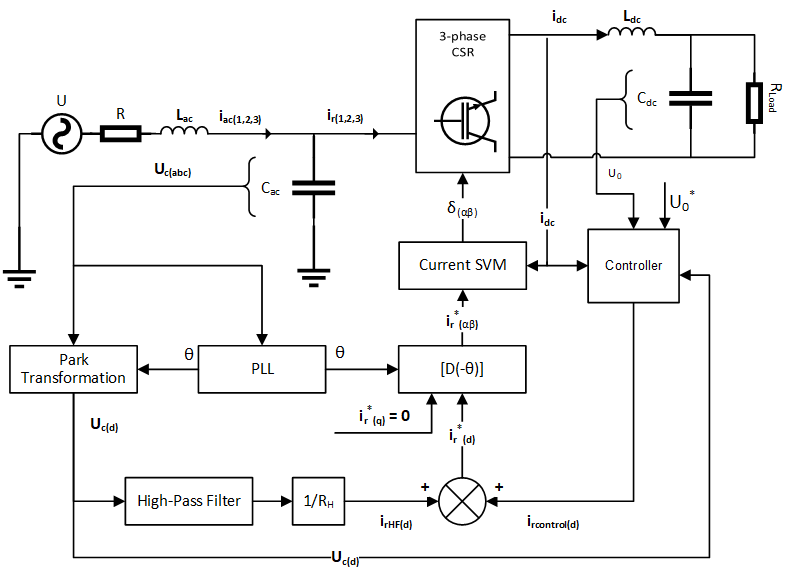
\includegraphics[width=\textwidth]{EMPC_PNG_Pics/ControlStructure.png}
        \caption{Block diagram of the control structure.}
        \label{EMPC:fig:ControlStruct}
    \end{figure}

    The controllers operate in the synchronous frame of the AC filter capacitor voltages $u_{c_{(1,2,3)}}$, and the rectifier input currents $i_{r_{(1,2,3)}}$ are in phase with the capacitor voltages.
    The current reference $i^*_{\alpha\beta}$ supplied to the space vector modulation unit in the stationary frame, is obtained by coordinate transformation $[D(-\Theta)]$ (or Park to Clarke transformation) of the current reference \ref{EMPC:equ:sync_ctrl} delivered by the current controllers in the synchronous frame.

    \begin{equation}
        \begin{array}{rcl}
            \begin{Bmatrix}
                i^*_{r_d}=i_{rcontrol_d}+i_{rHF_d}\\
                i^*_{r_q}=0
            \end{Bmatrix}
        \end{array}
        \label{EMPC:equ:sync_ctrl}
    \end{equation}

    In \ref{EMPC:equ:sync_ctrl}, $i_{rcontrol_d}$ represents the output of the DC voltage controller, while $i_{rHF_d}$ represents the damping current, proportional with the high frequency component of the filter capacitor voltage (the fundamental component of the capacitor voltage in the stationary frame becomes a DC component in the synchronous frame). The DC and AC side control units are explained in more detail in the following sections, and the performance of the control structure is evaluated.
		
\section{Control}\label{EMPC:sec:Control}

    In this section the model based control algorithm is explained, used on the DC side, followed by a simpler AC side active damping.

\subsection{DC-side explicit model predictive control} \label{EMPC:sec:DCside}

    Model predictive control (MPC) is an efficient and systematic method for solving complex multi-variable constrained optimal control problems \cite{vajda2017limiting}. The basic notions of MPC is explained in section \ref{BASICCSR:sec:MPC}, where the MPC control law is explained, namely, is based on the “receding horizon formulation”, where the model’s assumed behavior is calculated for a number of $N$ steps, where $N$ stands for the horizon’s length. Only the first step of the computed optimal input is applied in each iteration. The remaining steps of the optimal control input are discarded and a new optimal control problem (explained in section \ref{BASICCSR:sec:OptimalControl}) is solved at the next sample time. Using this approach, the receding horizon policy provides the controller with the desired feedback characteristics, although with high order systems the computational effort is considerably demanding since all the steps should be taken in to account on the specified horizon in every iteration.\\
		With Explicit MPC (EMPC), the discrete time constrained optimal control problem is reformulated as multi-parametric linear or quadratic programming. As explained in section \ref{BASICCSR:sec:EMPC}, the optimization problem can be solved offline, making it much more feasible from the perspective of the optimal control task. The optimal control law is a piecewise affine function of the states, and the resulting solution is stored in a pre-calculated lookup table. The parameter space, or the state-space is partitioned into critical regions. The real-time implementation consists in searching for the active critical region, where the measured state variables lie, and in applying the corresponding piecewise affine control law to achieve the desired dynamics.
    In order to introduce the MPC implementation from this paper, let us consider a linear discrete time system \ref{EMPC:equ:DiscreteStateSpace} derived with the discretisation of system \ref{EMPC:equ:mtx_DC} with zero-order hold method, where control inputs are assumed piecewise constant over the simulation sample time $T_s=\frac{1}{f_s}$ :

    \begin{equation}
        \begin{array}{rcl}
            \textbf{x}(t+1)&=&\textbf{A}_d\textbf{x}(t)+\textbf{B}_d\textbf{u}(t)\\
            \textbf{y}(t)&=&\textbf{C}_d\textbf{x}(t)
        \end{array}
        \label{EMPC:equ:DiscreteStateSpace}
    \end{equation}

    where $\textbf{A}_d$, $\textbf{B}_d$, $\textbf{C}_d$ are the matrices of the discretised system derived from \ref{EMPC:equ:mtx_ctrl}. With system \ref{EMPC:equ:DiscreteStateSpace} is linear and time invariant, MPC design can be followed. The following constraints have to be satisfied:

    \begin{equation}
        \begin{array}{r}
            \textbf{y}_{min}\leq\textbf{y}(t)\leq\textbf{y}_{max},\\
            \textbf{u}_{min}\leq\textbf{u}(t)\leq\textbf{u}_{max}
        \end{array}
        \label{EMPC:equ:contraint_desc}
    \end{equation}

    where $t>0$, $\textbf{x}\in \mathbb{R}^n$, $\textbf{u}\in \mathbb{R}^m$, $\textbf{y}\in \mathbb{R}^p$. The MPC solves the following constrained optimization problem \cite{rivera2013predictive}:

    \begin{equation}
        \begin{array}{rcl}
           \displaystyle \min_{U=\{u_t\dots u_t+N_u-1\}}J(\textbf{u},\textbf{x}(t))&=&\sum^{N_y-1}_{k=0}(\textbf{x}^T_{t+N_y|t}\textbf{Q_w}\textbf{x}_{t+N_y|t}+
           \textbf{u}^T_{t+k}\textbf{R_w}\textbf{u}_{t+k})\\
        \end{array}
        \label{EMPC:equ:optim_problem}
    \end{equation}

    subject to:

    \begin{equation}
        \begin{array}{l}
            \textbf{x}_{min}\leq\textbf{x}_{t+k|t}\leq\textbf{x}_{max},\,k=1,\dots,N_c-1\\
            \textbf{u}_{min}\leq\textbf{u}_{t+k|t}\leq\textbf{u}_{max},\,k=1,\dots,N_c-1\\
            \textbf{x}_{t|t}=\textbf{x}(t),\,\textbf{u}_{t|t}=\textbf{u}(t)\\
            \textbf{x}_{t+k+1|t}=\textbf{A}_d\textbf{x}_{t+k|t}+\textbf{B}_d\textbf{u}_{t+k|t}\\
            \textbf{y}_{t+k|t}=\textbf{C}_d\textbf{x}_{t+k|t}\\
            \textbf{u}_{t+k|t}=-K\textbf{x}_{t+k|t},\,k\geq0\\
        \end{array}
        \label{EMPC:equ:optim_problem_constr}
    \end{equation}
There the formulation of such problem is described in detail in chapter \ref{BASICCSR:sec:OptimalControl}.\\
    This problem is solved at each time instant $t$, where $\textbf{x}_{t+k\vert t}$ denotes the state vector predicted at time $t+k$, obtained by applying the input sequence $\textbf{u}_{t|t}...\textbf{u}_{t|t+1}$ to model \ref{EMPC:equ:quadratic_regions}, starting from the state $\textbf{x}_{t|t}$. Further, it is assumed that $Q$ and $R$, are symmetric positive semidefinite $(\textbf{Q}_w=\textbf{Q}_w^T\geq0$, $\textbf{R}_w=\textbf{R}_w^T>0)$ and $K$ is a feedback gain. Further, $N_y,N_u,N_c$ are the output, input and constraint horizons, respectively.
    Using the model for predicting the future behavior of the system and with some appropriate substitution and variable manipulation which basic notions showed in section \ref{BASICCSR:sec:MPC}, the problem \ref{EMPC:equ:optim_problem},\ref{EMPC:equ:optim_problem_constr} can be transformed to the standard multi parametric quadratic programming form, as described in \cite{rivera2013predictive}:
%
%    \begin{equation}
%        \begin{array}{rcl}
%            J(\textbf{x}(t))&=&\min \textbf{z}'\textbf{H}\textbf{z}
%        \end{array}
%        \label{EMPC:equ:quadratic_program}
%    \end{equation}

    \begin{equation}
        \begin{array}{rcl}
            J^*(\textbf{x}(t))&=&\min_{\textbf{z}}J(\textbf{x},\textbf{z})=\frac{1}{2}\textbf{z}'\textbf{H}\textbf{z}
        \end{array}
        \label{EMPC:equ:quadratic_program}
    \end{equation}

    where subject to:

    \begin{equation}
        \begin{array}{rcl}
            \textbf{Gz}&\leq&\textbf{W}+\textbf{S}\textbf{x}(t)
        \end{array}
        \label{EMPC:equ:quadratic_inequality}
    \end{equation}

    where the matrices $\textbf{H}$, $\textbf{G}$, $\textbf{W}$, $\textbf{S}$ result directly from the coordinate transformations described in \ref{BASICCSR:sec:OptimalControl}. The solution of the quadratic optimization problem for each critical region has the form:

    \begin{equation}
        \begin{array}{rcl}
            \textbf{u}^*&=&f_i\textbf{x}+g_i
        \end{array}
        \label{EMPC:equ:quadratic_regions}
    \end{equation}

    and the critical region is described by:

    \begin{equation}
        \begin{array}{rcl}
            \mathcal{C}_{reg_i}&=&\{\textbf{x}\in mathbb{R}^n|\textbf{H}_i\textbf{x}\leq K_i\}
        \end{array}
        \label{EMPC:equ:quadratic_critical}
    \end{equation}

    Thus, the explicit MPC controller is completely characterized by the set of parameters:

    \begin{equation}
        \begin{array}{l}
            \{f_i,g_i,\textbf{H}_i,\textbf{K}_i|i=1\dots N\}
        \end{array}
        \label{EMPC:equ:quadratic_set}
    \end{equation}

    In case of the discrete time system resulting from \ref{EMPC:equ:mtx_ctrl}, for sampling time equal with the switching period $T_s=5\cdot10^{-5}$  s, the problem defined to be solved by MPC is the minimization of the quadratic cost function \ref{EMPC:equ:DiscreteStateSpace} for:

    \begin{equation}
        \begin{array}{l}
            \textbf{R}_w=\begin{bmatrix}
                1& 0\\
                0& 1\\
            \end{bmatrix},
            \textbf{Q}_w=\begin{bmatrix}
                10^{-6}& 0\\
                0& 10^{-6}\\
            \end{bmatrix},
            N_y=N_u=N_c=2
        \end{array}
        \label{EMPC:equ:quadratic_mtx_set}
    \end{equation}

    Since $N_y,N_u,N_c$ take the same value, they will be substituted by $N$.
    The constraints defined based on the rated power of the CSR $P_n=2500$ W, are:

    \begin{equation}
        \begin{array}{rcl}
            0\leq&i_{dc}&\leq 50A\\
            0\leq&u_{0}&\leq 500V
        \end{array}
        \label{EMPC:equ:numeric_constraints}
    \end{equation}

    The state space partition resulting from this problem has 13 critical regions, which can be observed in Fig. \ref{EMPC:fig:regions}.

    \begin{figure}[!ht]
        \centering
        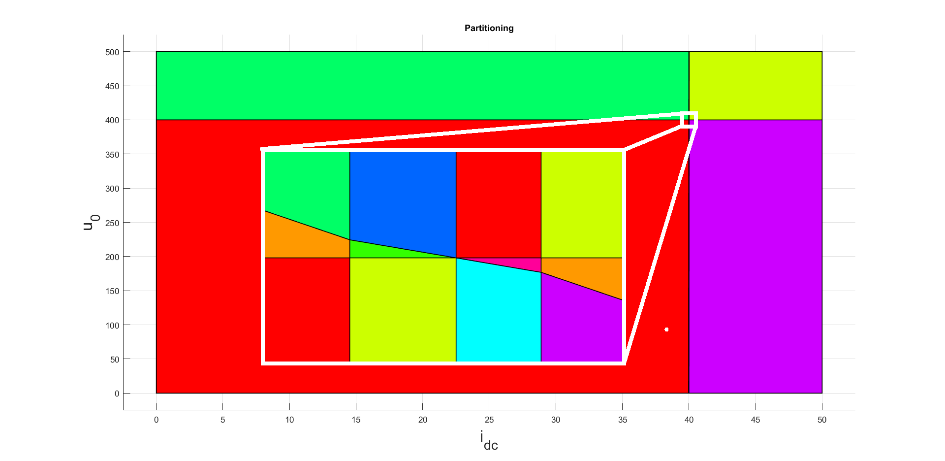
\includegraphics[width=\textwidth]{EMPC_PNG_Pics/Regions.png}
        \caption{State space partitioning.}
        \label{EMPC:fig:regions}
    \end{figure}

    From the basis of the discretised model \ref{EMPC:equ:DiscreteStateSpace}, the given constraints \ref{EMPC:equ:numeric_constraints}, and horizon \ref{EMPC:equ:numeric_constraints} the cost function \ref{EMPC:equ:optim_problem} is established via the MPT toolbox [30] and used in the generated controller for the EMPC design [29], [31]. The controller is created as a compliable S-function in the Matlab/Simulink environment and its place in the control structure can be observed in Fig. \ref{EMPC:fig:MPCStructure}. as the EMPC controller.
    The output of the MPC controller is the control variable obtained via solving \ref{EMPC:equ:optim_problem_constr} and
    $u_{MPC}=(\delta_du_{c_d}+\delta_qu_{c_q})$, from which the current reference can be calculated using \ref{EMPC:equ:numeric_constraints}. The quadrature component $u_{c_q}$ is zero in the synchronous frame of the filter capacitor voltage.


    \begin{equation}
        \begin{array}{rcl}
            i_{rMPC_{d}}&=&\frac{u_{MPC}}{u_{c_d}}\cdot i_{dc}
        \end{array}
        \label{EMPC:equ:direct_controlval}
    \end{equation}

    \begin{figure}[!ht]
        \centering
        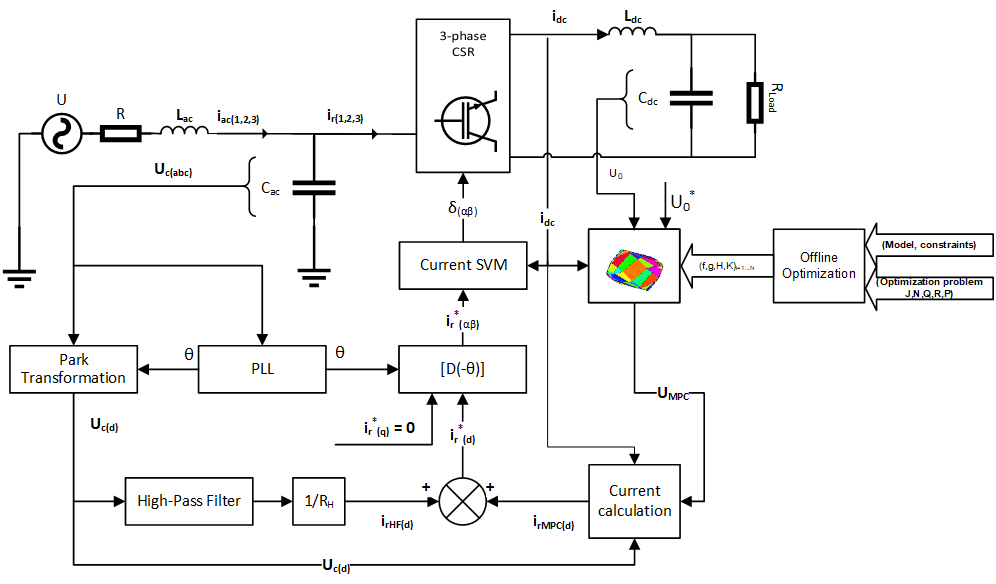
\includegraphics[width=\textwidth]{EMPC_PNG_Pics/MPCStructure.png}
        \caption{The control structure of the CSR, with MPC controller on the DC side.}
        \label{EMPC:fig:MPCStructure}
    \end{figure}

\subsection{Active AC-side damping}\label{EMPC:sec:ACdamping}

    The CSR requires a voltage supply on the AC side. Taking the inductive character of the mains into consideration, the presence of a three-phase capacitor bank at the input of the CSR is a must. The most convenient is to use three-phase LC filtering with inductors on the lines and star connected capacitors resembling those in Fig. \ref{EMPC:fig:network}, although the resonance phenomena between these components can still cause difficult problems. The simplest way to dampen the resonance on the AC side LC filter is to add a damping resistor across the capacitor \cite{regaya2014new}. Because these resistors result in high losses, active damping methods have been proposed, which emulate damping resistors by control. This makes the CSR bridge produce an additional high frequency current, equivalent to the presence of virtual damping resistors connected in parallel with the AC capacitors. The resonance of the AC side LC filter produces harmonics in the capacitor voltage with frequency close to $\omega_{ac}=\frac{1}{\sqrt{L_{ac}C_{ac}}}$, which appears as $\omega_{ac}-\omega$ component in $u_{c_d}$, where $\omega=2\pi f$. The fundamental component of the capacitor voltage represents a DC component in the synchronous reference frame. Therefore, a high-pass filter (HPF) is applied to filter out this DC component, with the transfer function:

    \begin{equation}
        \begin{array}{rcl}
            HPF(s)&=&\frac{s}{s+0.1\cdot(\omega_{ac}-\omega}
        \end{array}
        \label{EMPC:equ:AC_HPF}
    \end{equation}

    A virtual damping resistance $R_H$ has been defined for calculation of the damping current component $i_{HPF}$ from the HPF component of the capacitor voltage.

\section{Modulation}\label{EMPC:sec:Modulation}

    The chosen modulation strategy is developed in the $"\alpha\beta"$ stationary reference frame, based on the notions already mentioned in section \ref{BASICCSR:sec:OperationPrinciple}. The structure requires simultaneous conduction of the upper and lower transistors of the bridge, since the current of the $L_{dc}$  choke must not be interrupted. Additionally, the switching devices are considered as ideal.

    \begin{figure}[!ht]
        \centering
        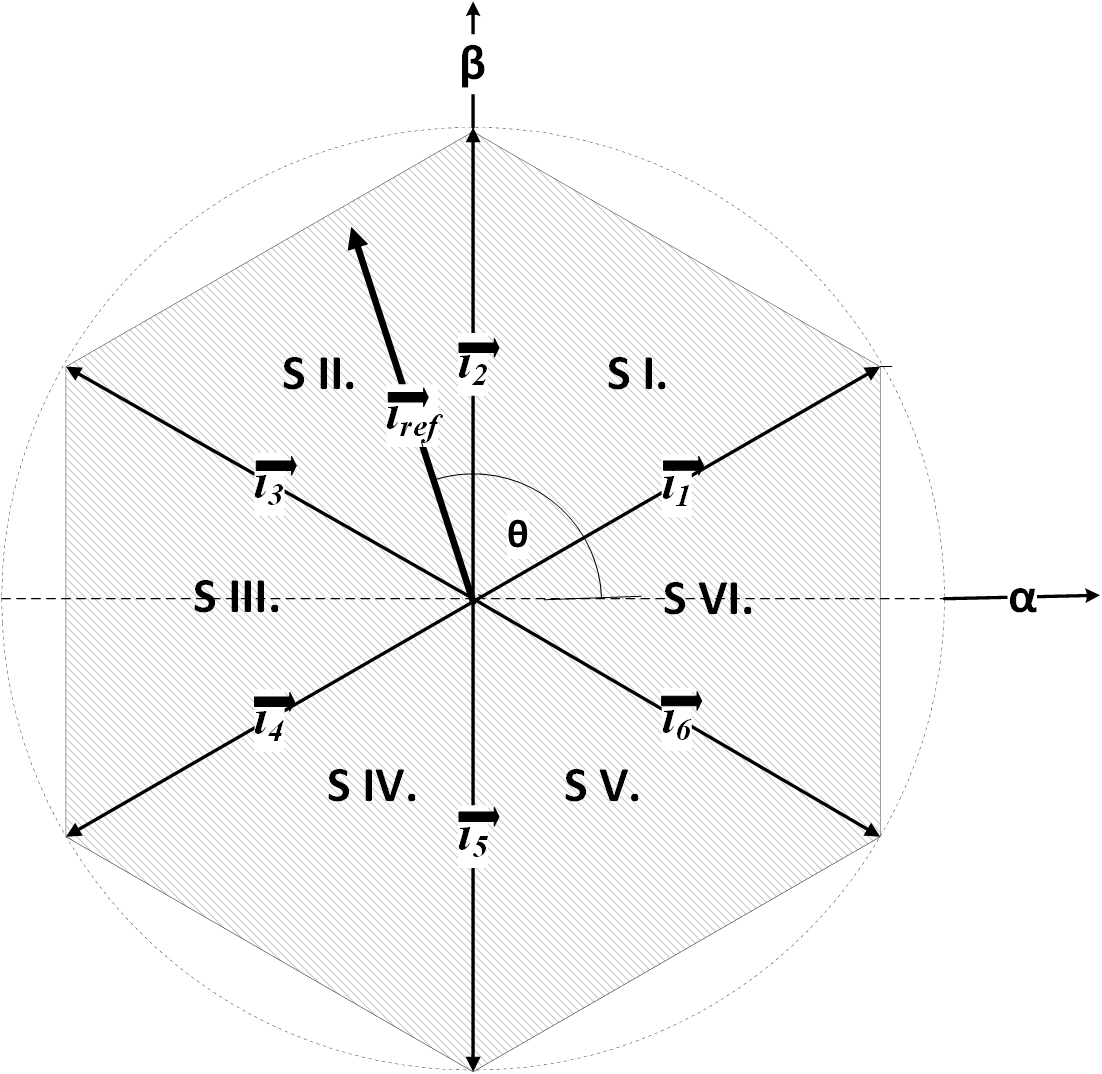
\includegraphics[width=.6\textwidth]{EMPC_PNG_Pics/VectorPhasor.png}
        \caption{The fundamental input current vectors corresponding to the active switching states of the CSR.}
        \label{EMPC:fig:VectorPhasor}
    \end{figure}

    According to this, one of the upper and one of the lower switches must be closed at all times. This allows nine states, six of which are active. There are three "zero" vectors, corresponding to the switching states, when both devices of one of the bridge legs are in conduction. These current vectors are shown in Table \ref{EMPC:tbl:fundamental_vect}.


% Please add the following required packages to your document preamble:
% \usepackage{multirow}
% \usepackage[table,xcdraw]{xcolor}
% If you use beamer only pass "xcolor=table" option, i.e. \documentclass[xcolor=table]{beamer}

\begin{table}[]
\caption{The fundamental input current vectors corresponding to the active switching states of the CSR.}
    \begin{tabular}{|l|l|l|l|l|l|l|l|l|l|l|}
    \hline
    \rowcolor[HTML]{EFEFEF}
    \multicolumn{1}{|c|}{\cellcolor[HTML]{EFEFEF}}                                & \multicolumn{6}{c|}{\cellcolor[HTML]{EFEFEF}\textbf{Switching State}}       & \multicolumn{3}{l|}{\cellcolor[HTML]{EFEFEF}\textbf{Phase currents}} & \multicolumn{1}{c|}{\cellcolor[HTML]{EFEFEF}}                                                 \\ \cline{2-10}
    \rowcolor[HTML]{EFEFEF}
    \multicolumn{1}{|c|}{\multirow{-2}{*}{\cellcolor[HTML]{EFEFEF}\textbf{Name}}} & \textbf{1} & \textbf{2} & \textbf{3} & \textbf{4} & \textbf{5} & \textbf{6} & \textbf{ia}           & \textbf{ib}           & \textbf{ic}          & \multicolumn{1}{c|}{\multirow{-2}{*}{\cellcolor[HTML]{EFEFEF}\textbf{Vector representation}}} \\ \hline
    $\vec{i}_1$                                                                           & 1          & 0          & 0          & 0          & 0          & 1          & $i_{dc}$                   & 0                     & -$i_{dc}$                 & $2i_{dc}e^{j\pi/6}/\sqrt{3}$                                                                                           \\ \hline
    $\vec{i}_2$                                                                            & 0          & 0          & 1          & 0          & 0          & 1          & 0                     & $i_{dc}$                   & -$i_{dc}$                 & $2i_{dc}e^{j\pi/2}/\sqrt{3}$                                                                                           \\ \hline
    $\vec{i}_3$                                                                            & 0          & 1          & 1          & 0          & 0          & 0          & -$i_{dc}$                  & $i_{dc}$                   & 0                    & $2i_{dc}e^{j5\pi/6}/\sqrt{3}$                                                                                          \\ \hline
    $\vec{i}_4$                                                                            & 0          & 1          & 0          & 0          & 1          & 0          & -$i_{dc}$                  & 0                     & $i_{dc}$                  & $2i_{dc}e^{j7\pi/6}/\sqrt{3}$                                                                                          \\ \hline
    $\vec{i}_5$                                                                           & 0          & 0          & 0          & 1          & 1          & 0          & 0                     & -$i_{dc}$                  & $i_{dc}$                  & $2i_{dc}e^{j3\pi/2}/\sqrt{3}$                                                                                           \\ \hline
    $\vec{i}_6$                                                                            & 1          & 0          & 0          & 1          & 0          & 0          & $i_{dc}$                   & -$i_{dc}$                  & 0                    & $2i_{dc}e^{j11\pi/6}/\sqrt{3}$                                                                                           \\ \hline
    $\vec{i}_7$                                                                            & 1          & 1          & 0          & 0          & 0          & 0          & 0                     & 0                     & 0                    & 0                                                                                             \\ \hline
    $\vec{i}_8$                                                                            & 0          & 0          & 1          & 1          & 0          & 0          & 0                     & 0                     & 0                    & 0                                                                                             \\ \hline
    $\vec{i}_9$                                                                            & 0          & 0          & 0          & 0          & 1          & 1          & 0                     & 0                     & 0                    & 0                                                                                             \\ \hline
    \end{tabular}
        \label{EMPC:tbl:fundamental_vect}

\end{table}

    The neighboring space phasors can be formulated as:

    \begin{equation}
        \begin{array}{rcl}
            \vec{i}_n&=&\frac{2}{\sqrt{3}}i_{dc}e^{j(\frac{n\pi}{3}-\frac{\pi}{6})}\\
            \vec{i}_{n+1}&=&\frac{2}{\sqrt{3}}i_{dc}e^{j(\frac{n\pi}{3}+\frac{\pi}{6})}\\
            n&=&1,2,\dots,6
        \end{array}
        \label{EMPC:equ:neighbor}
    \end{equation}

    The reference current vector is sampled with fixed sampling period $T_s$. The sampled value of $\overrightarrow{i_{ref}}$ is synthesized as the time average of two neighbouring space phasors adjacent to the reference current:

    \begin{equation}
        \begin{array}{rcl}
            T_n\vec{i}_n+T_{n+1}\vec{i}_{n+1}&=&T_s\vec{i}_{ref}
        \end{array}
        \label{EMPC:equ:i_ref}
    \end{equation}

    $T_n$ and $T_{n+1}$ represent the individual durations of the switching states corresponding to the neighboring vectors. For example, in case of a current reference vector situated in the first sector, $T_1$, $T_2$ and $T_0$ can be calculated using \ref{EMPC:equ:dwelltime}.

    \begin{equation}
        \begin{array}{rcl}
            T_1&=&T_s\frac{i_{ref_\alpha}}{i_{dc}}\\
            T_2&=&T_s\frac{\sqrt{3}}{2i_{dc}}(i_{ref_\beta}-\frac{i_{ref_\alpha}}{\sqrt{3}})\\
            t_0&=&T_s-T_n-T_{n-1}=T_{7,8,9}
        \end{array}
        \label{EMPC:equ:dwelltime}
    \end{equation}

    \begin{figure}[!ht]
        \centering
        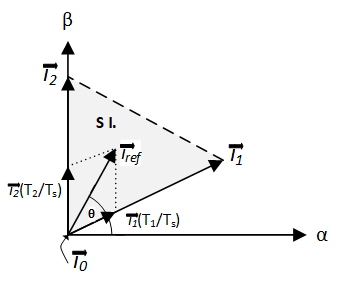
\includegraphics[width=0.6\textwidth]{EMPC_PNG_Pics/OnePhasor.png}
        \caption{Synthesis of $\protect\overrightarrow{i_{ref}}$ by $\protect\overrightarrow{i_{1}}$, $\protect\overrightarrow{i_{2}}$, and $\protect\overrightarrow{i_{0}}$}
        \label{EMPC:fig:OnePhasor}
    \end{figure}

    The complex plane is naturally divided by the fundamental space vectors into six areas, named "sectors".

    \begin{equation}
        \begin{array}{l}
            x\frac{\pi}{6}+\frac{(n-1)\pi}{3}\leq\theta_n\leq\frac{\pi}{6}+\frac{n\pi}{3}\\
            n=1,2,\dots,6
        \end{array}
        \label{EMPC:equ:angle}
    \end{equation}

    The non-zero space vectors are selected based on the phase angle $\theta$ between $\overrightarrow{i_{ref}}$ and the real axis.
    Table \ref{EMPC:tbl:sequence} presents an example of switching pattern in case of a current reference vector situated in Sector I.

    \begin{table}[]

		\caption{Representation of switching sequences for SECTOR I.}
		\centering
        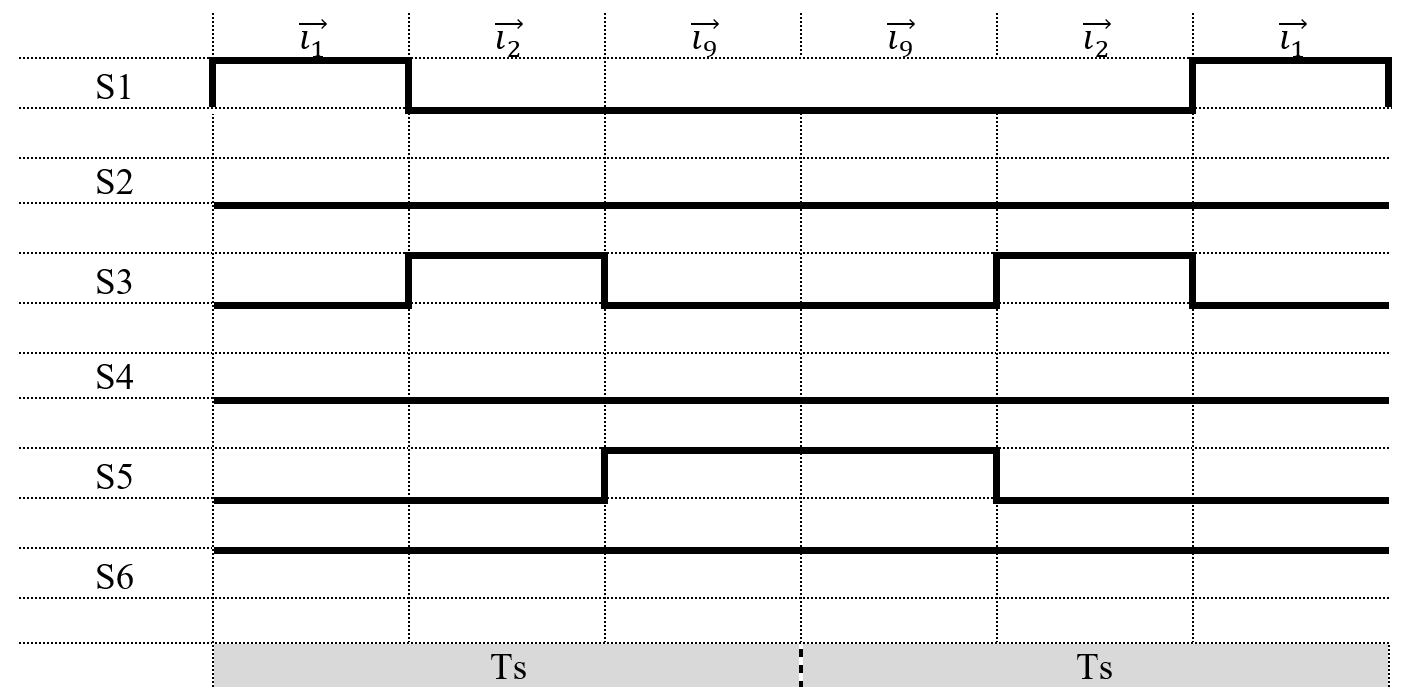
\includegraphics[width=0.8\textwidth]{EMPC_PNG_Pics/Sequence.png}

        \label{EMPC:tbl:sequence}
    \end{table}

    The switching scheme represented in Table \ref{EMPC:tbl:fundamental_vect}. is aimed at reducing the number of commutations in a switching cycle, resulting in the reduction of the switching losses \cite{moussaoui2005open}.
    Additionally, the constraint (\ref{EMPC:equ:refconstraint}) resulting from the available magnitudes of the current vectors, is applied to the current reference.

    \begin{equation}
        \begin{array}{l}
            0\leq|i_{ref}|\leq\frac{\sqrt{6}i_{dc}}{cos\theta+\sqrt{3}sin\theta}
        \end{array}
        \label{EMPC:equ:refconstraint}
    \end{equation}

\section{Discussion}\label{EMPC:sec:Discussion}

    From the continuous AC \ref{EMPC:equ:mtx_AC}, and DC \ref{EMPC:equ:mtx_DC} model equations described in Ch.X., the controller is formulated form discretised system \ref{EMPC:equ:DiscreteStateSpace}, and it is described via the cost function and control problem of \ref{EMPC:equ:optim_problem}, and \ref{EMPC:equ:optim_problem_constr} in Ch.X$+$1. The evaluated model and control structure are shown on Fig.4. In the following section said EMPC’s computational requirements are evaluated, and the Matlab/Simulink simulation results are compared to a classic state feedback controller’s dynamic performance.

    \subsection{Computational effort}\label{EMPC:sec:CompEffort}

    The binary search tree generated for the control problem presented in Fig. \ref{EMPC:fig:SearchTree}. The search method and formulation of the tree is described in chapter \ref{BASICCSR:sec:EMPCStorage}. The depth of the search tree is 5 and it has a total number of 29 nodes. It is utilized with the MPT toolbox \cite{muthukumar2016adaptive}, \cite{kutasi2010constrained}, and it can be used for the computationally optimal real-time implementation of the proposed algorithm on low-cost hardware.

    \begin{figure}[!ht]
        \centering
        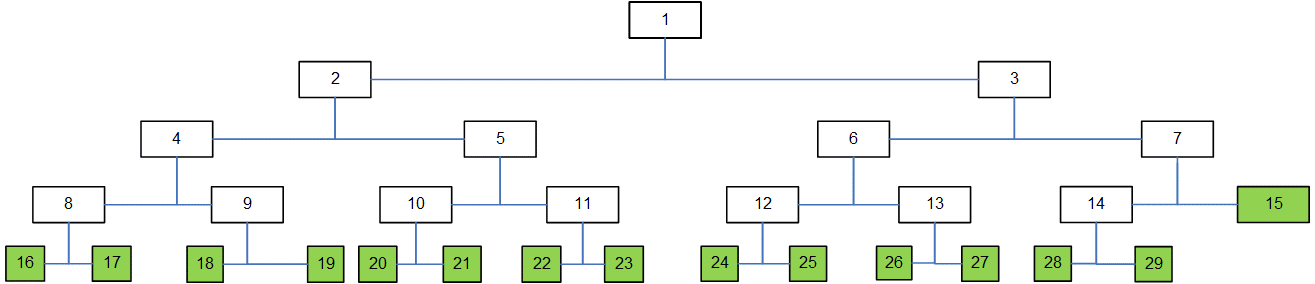
\includegraphics[width=\textwidth]{EMPC_PNG_Pics/SearchTree.png}
        \caption{Binary search tree of the controller for a horizon of $N = 4$. The leaf nodes are depicted with filled squares. The depth of the tree is 5.}
        \label{EMPC:fig:SearchTree}
    \end{figure}

    The search for an active critical region starts from the first level and represents the evaluation in each adjacent node of an inequality of the form: $x\leq K$. Thus, in this case a maximum number of 4 inequalities have to be evaluated to reach the active critical region. Implementing the presented algorithm is straightforward on a DSP processor, for instance from the dsPIC33 family by Microchip. Using the MAC (multiply and accumulate) instruction the inequality is evaluated for each node using 4 instructions, thus in 80 ns on a 50 MIPS processor (Fig. \ref{EMPC:fig:Memory}). The active critical region can be reached in a maximum of 400 ns. Compared to the typical sample rate of 10us in the case of a CSR, the real-time implementation on a DSP processor is possible.

   % \begin{table}[]
%\caption{asd}
%    \begin{tabular}{ccc}
%    asd
%    &asd
%    &asd    \\
%    \end{tabular}
%    \end{table}

    \begin{figure}[!ht]
        \centering
        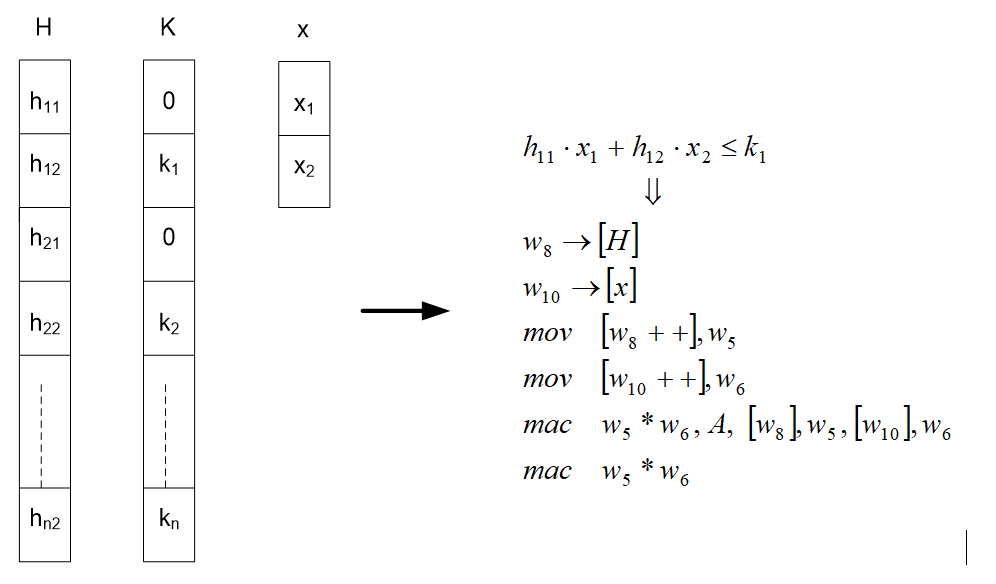
\includegraphics[width=\textwidth]{EMPC_PNG_Pics/Memory.png}
        \caption{Data organization in the data memory of a single core DSP and the evaluation of a 2-dimensional inequality}
        \label{EMPC:fig:Memory}
    \end{figure}

    \subsection{Horizon performance}\label{EMPC:sec:Performance}

    With the cost function (\ref{EMPC:equ:optim_problem}) employed using (\ref{EMPC:equ:quadratic_mtx_set}), changing the length of the horizon ($N$) affects the system's complexity illustrated by the partition in the state space shown in Fig. \ref{EMPC:fig:regions}., and Fig. \ref{EMPC:fig:MultiHorizon} presents the step response of the controlled system for different lengths of the horizon. It shows, that the response is not affected by the increase of the horizon above $N=2$, supporting the choice of this value for Matlab Simulink implementation.

    \begin{figure}[!ht]
        \centering
        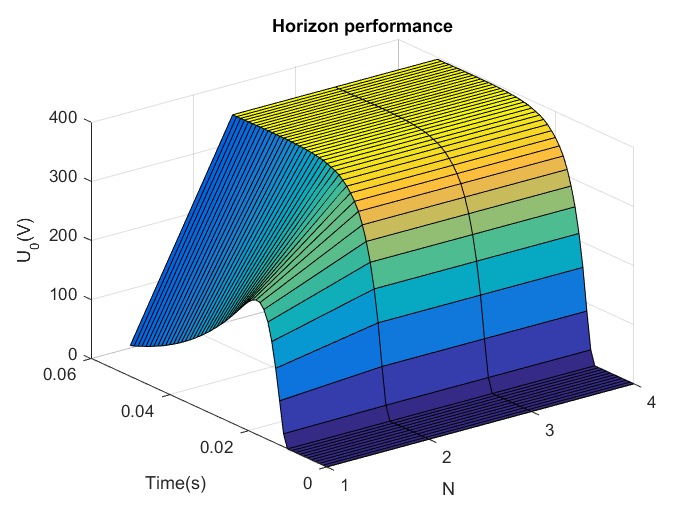
\includegraphics[width=\textwidth]{EMPC_PNG_Pics/MultiHorizon.png}
        \caption{Step response of the system as a function of the horizon length (N).}
        \label{EMPC:fig:MultiHorizon}
    \end{figure}

    \subsection{Simulation results}\label{EMPC:sec:Results}

    The simulation results are produced with Matlab/Simulik. The discrete model's (\ref{EMPC:equ:DiscreteStateSpace}) simulation frequency was 1 MHz, with the model parameters represented in Table \ref{EMPC:tbl:params}., and with the control structure shown on Fig. \ref{EMPC:fig:ControlStruct}. The EMPC performance is shown below:

    \begin{figure}[!ht]
        \centering
        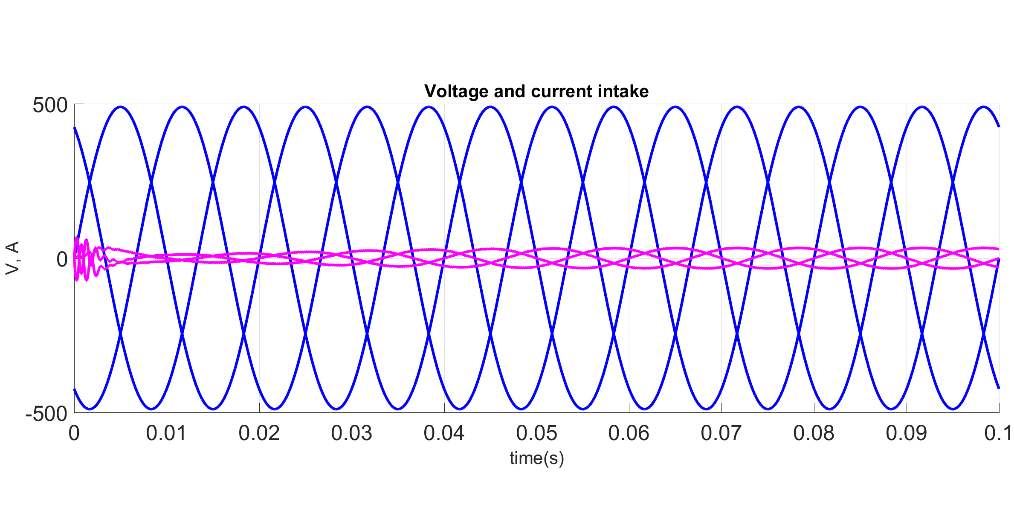
\includegraphics[width=\textwidth]{EMPC_PNG_Pics/Result_3fEMPC.png}
        \caption{Three-phase voltage and current intake of the CSR with EMPC}
        \label{EMPC:fig:Result_3fEMPC}
    \end{figure}

    \begin{figure}[!ht]
        \centering
        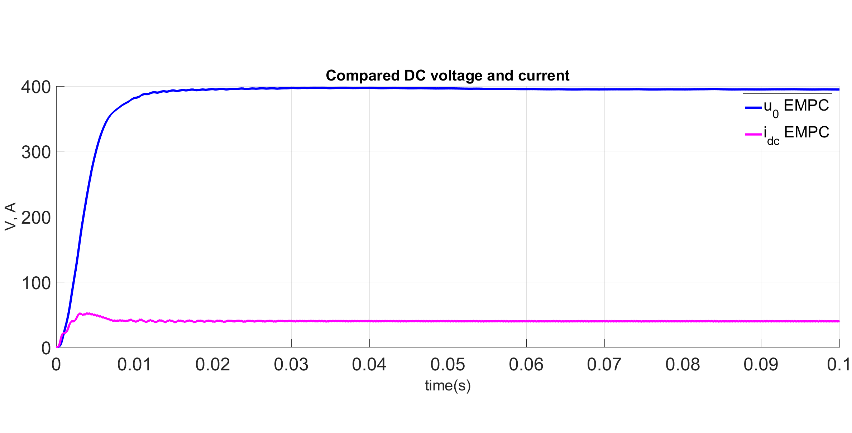
\includegraphics[width=\textwidth]{EMPC_PNG_Pics/Result_PerformanceEMPC.png}
        \caption{Resulting current and voltage trajectories of the CSR with (EMPC).}
        \label{EMPC:fig:Result_PerformanceEMPC}
    \end{figure}

    More details about the Matlab simulation are presented in \cite{neukirchner2019linkedmodel}.

    \subsection{Comparison with a state feedback control}\label{EMPC:sec:Comparison}

    On the DC side, not only the output voltage $u_0$ but also the inductor current $i_{dc}$ needs to be controlled. Described in [28], a state feedback control with optimal parameters can be used as a reference based on the model properties listed in Table \ref{EMPC:tbl:params}, with output voltage $u_0$ and DC bus current $i_{dc}$ chosen as the state variables. Since $u_0$ is a DC quantity in steady state, an integrator signal is introduced to diminish the steady-state error. The structure of the controller is represented in Fig. \ref{EMPC:fig:SFeedbackDC}.

    \begin{figure}[!ht]
        \centering
        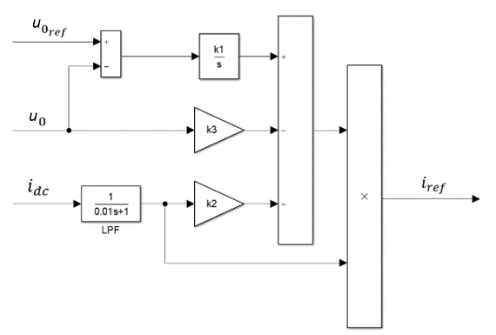
\includegraphics[width=0.7\textwidth]{EMPC_PNG_Pics/SFeedbackDC.png}
        \caption{Simple DC side state feedback control structure.}
        \label{EMPC:fig:SFeedbackDC}
    \end{figure}

    The tuning constants applied and calculated according to \cite{godlewska2015predictive} are:

    \begin{equation}
        \begin{array}{l}
            k1=\frac{\omega^3_n}{1.5U_n\omega^2_{dc}},\,k2=\frac{1.9\omega_n L_{dc}}{1.5U_n},\,k3=\frac{2.2\omega^2_n}{1.5U_n(\omega^2_{dc}-1)},\\
            \textnormal{where,}\\
            \omega_n=1.1,\,\omega_{ac}=\frac{1}{\sqrt{L_{ac}C_{ac}}},\,\omega_{dc}=\frac{1}{\sqrt{L_{dc}C_{dc}}}
        \end{array}
        \label{EMPC:equ:tuning}
    \end{equation}

    The state feedback controllers block on the diagram is taking the controller's place, shown on Fig. \ref{EMPC:fig:ControlStruct}. The independent outputs are the high pass filter's output  $i_{rHPF(d)}$ and the controller's output $i_{rcontrol(d)}$. The sum of the independent current values is converted to Clarke frame to be able to govern the switching states of the IGBT's. This can be done because $i_{rHF(d)}$ has only high frequency components and $i_{rcontrol(d)}$ has low frequency components due to the differences in LC time constants, as discussed in the second section. Then the control signal governing the switches is applied in the same manner, described at the start of section \ref{EMPC:sec:Modulation}.
    The state feedback control's performance in comparison with the EMPC is shown in Fig. \ref{EMPC:fig:Result_EMPCfinal}.

    \begin{figure}[!ht]
        \centering
        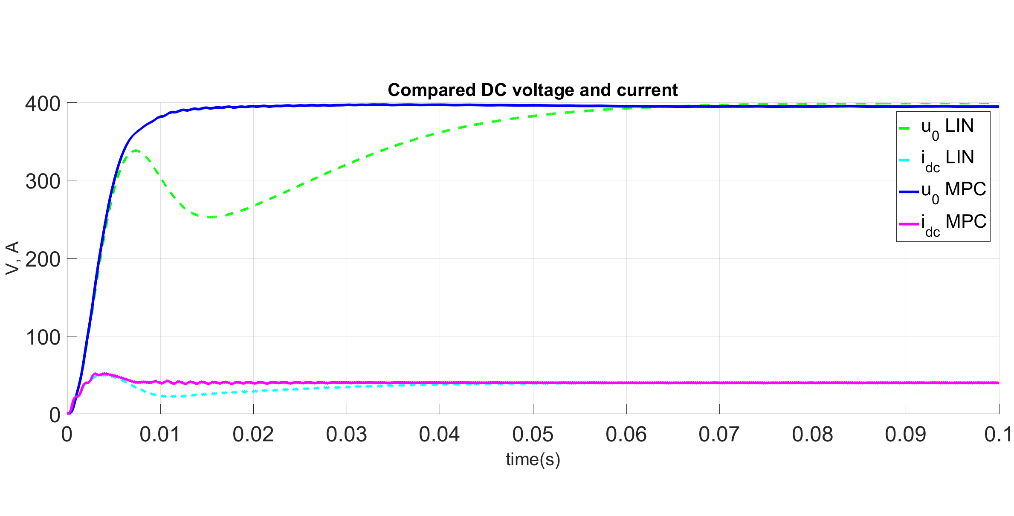
\includegraphics[width=\textwidth]{EMPC_PNG_Pics/Result_EMPCfinal.png}
        \caption{Resulting current and voltage trajectories of the CSR with explicit model predictive control (MPC) compared state feedback control (LIN).}
        \label{EMPC:fig:Result_EMPCfinal}
    \end{figure}

\section{Conclusion}\label{EMPC:sec:Conclusions}

    The constrained, model-based optimal control of a current source rectifier has been presented in this paper. The dynamic model of a three-phase current source rectifier has been developed in Park frame. The proposed model has been examined from the design and implementation points of view with the purpose of explicit model-based predictive control. It proved to be the case that the regular set of differential equations of the CSR appears to be too complex, and contains non-linearity for such a design approach. To address this issue the usage of separated AC and DC equation sets was suggested to avoid linearization and complexity reduction. This solution eliminates bilinearity and enables the application of linear control design techniques. Current-based SVPWM of the three-phase converter has been used with an emphasis on the reduction of switching losses. Throughout the article the explicit model predictive control method is described and the method's effectiveness compared to conventional state feedback control is show. The implementation and simulation experiments have been performed in Matlab/Simulink environment. Moreover, the proper implementation of the system in a modern DSP chip will result in real-time operation.
		
		\section{Notations}
		
		%\begin{longtable}{r|l}
  % after \\: \hline or \cline{col1-col2} \cline{col3-col4} ...
  %Chapter 4.1. notations&\\
  \begin{scriptsize}
\begin{tabularx}{\textwidth}{r|X}
  $\textbf{A}$                  & State matrix of the DC side system\\
  $\textbf{A_d}$                & Discretised state matrix of the DC side system\\
  $\textbf{B}$                  & Input matrix of the DC side system\\
  $\textbf{B_d}$                & Discretised input matrix of the DC side system\\
  $C_{ac}$                          & AC side inductance\\
  $C_{dc}$                          & DC side inductance\\
  $\textbf{C}$                  & Output matrix of the DC side system\\
  $\textbf{C_d}$                & Discretised output matrix of the DC side system\\
  $C_{reg_i}$                       & Critical region\\
  $D(-\Theta)$                      & Inverse Clarke transformation\\
  $f$                               & Network voltage frequeny\\
  $fpwm$                            & Rectifier switching frequency\\
  $f_s$                             & Simulation frequency\\
  $f_i$                             & Function of state at the $i^th$ step\\
  $g_i$                             & Function of input at the $i^th$ step\\
  $G$                               & Constraint input matrix\\
  $H$                               & Supplementary matrix\\
  $HPF(s)$                          & High pass filter transfer function\\
  $i_{ac_{1,2,3}}$                  & AC side inductance current\\
  $i_{ac_{\alpha,\beta}}$           & AC side inductance current in Clarke frame\\
  $i_{ac_{d,q}}$                    & AC side inductance current in Park frame\\
  $i_{HPF}$                         & AC side damping current\\
  $i_{r_{1,2,3}}$                   & Rectifier current\\
  $i_{rMPC_d}$                      & Direct component of the output of the EMPC controller\\
  $i^*_{r_{1,2,3}}$                 & Rectifier reference current\\
  $i^*_{r_{\alpha,\beta}}$          & Rectifier reference current in Clarke frame\\
  $i_{rcontrol_d}$                  & Direct component of the output of the DC voltage controller\\
  $i_{rHF_d}$                       & Direct component of the damping current of AC noise\\
  $i_{dc}$                          & DC side inductance current\\
  $i_{ref_{\alpha,\beta}}$          & $\alpha$, or $\beta$ component of the reference current vector respecively\\
  $\vec{i}_{0,\dots,9}$             & Current vector of the phasor\\
  $\vec{i}_{ref}$                   & Reference current vector\\
  $J$                               & Quadratic EMPC cost function\\
  $J^*$                             & Optimal cost value\\
  $k_{1,2,3}$                       & State feedback controller's coefficients\\
  $K$                               & Feedback gain of EMPC controller\\
  $L_{ac}$                          & AC side inductance\\
  $L_{dc}$                          & DC side inductance\\
  $n$                               & Current phasor sector indicator\\
  $N$                               & Control horizon\\
  $N_y,N_u,N_c$                     & Output, input and constraint horizons\\
  $P_n$                             & Nominal power of the CRS\\
  $\textbf{Q}_w$                & State weight matrix of quadratic MPC cost function\\
  $R$                               & Phase resistance\\
  $R_H$                             & Virtual damping resistance\\
  $R_{load}$                        & Load resistance\\
  $\textbf{R}_w$                & Input weight matrix of quadratic MPC cost function\\
  $\mathbb{R}$                      & Set of real numbers\\
  $S$                               & Current phasor sector\\
  $\textbf{S}$                  & Coefficient constraint matrix\\
  $t$                               & Discrete timestep\\
  $T_s$                             & Switching period\\
  $T_{0,\dots,9}$                   & Dwell time in the corresponding sector\\
  $\textbf{u}$                  & Output vector of the DC side system\\
  $u_{1,2,3}$                       & AC side phase voltage\\
  $u_{\alpha,\beta}$                & AC side phase voltage in Clarke frame\\
  $u_{d,q}$                         & AC side phase voltage in Park frame\\
  $u_{c_{1,2,3}}$                   & AC side capacitance voltage\\
  $u_{c_{\alpha,\beta}}$            & AC side capacitance voltage in Clarke frame\\
  $u_{c_{d,q}}$                     & AC side capacitance voltage in Park frame\\
  $u_0$                             & DC side voltage on load\\
  $u^*_0$                           & DC side voltage reference\\
  $u_{MPC}$                         & MPC control variable\\
  $\textbf{u}^*$                & Optimal input vector\\
  $U$                               & Set of MPC inputs\\
  $Un$                              & Network line-to-line voltage\\
  $\textbf{x}$                  & State vector of the DC side system\\
  $\textbf{y}$                  & Input vector of the DC side system\\
  $\textbf{z}$                  & Vector of optimization variables\\
  $\delta_{1,2,3}$                  & Conduction state leg in Clarke frame\\
  $\delta_{\alpha,\beta}$           & Conduction state leg in Park frame\\
  $\delta_{d,q}$                    & Conduction state leg\\
  $\theta$                          & Network voltage vector’s angular displacement\\
  $\omega$                          & Network voltage vector’s angular velocity\\
  $\omega_{ac}$                     & Ac side LC filter angular velocity\\
  $\omega_{n}$                      & Damping angular velocity\\
  \end{tabularx}
  \end{scriptsize}
%\hline
%\end{longtable}
		
